\documentclass[12pt]{article}

% Настройка русского языка и шрифтов
\usepackage[utf8]{inputenc}
\usepackage[russian]{babel}
\usepackage[T2A]{fontenc}

% Математические пакеты
\usepackage{amsmath, amssymb, amsfonts}

% Настройка страницы
\usepackage{geometry}
\geometry{a4paper, margin=0.8in}

% Другие полезные пакеты
\usepackage{hyperref}
\usepackage{booktabs}
\usepackage{enumitem}
\usepackage{longtable}
\usepackage{graphicx}
\usepackage{xcolor}

% Определение стилей для комментариев
\definecolor{commentgray}{rgb}{0.4,0.4,0.4}
\definecolor{antigravityblue}{rgb}{0.0, 0.45, 0.74}

\newcommand{\commentary}[1]{{\small\itshape\color{commentgray} #1}}
\newcommand{\antigravity}[1]{{\small\color{antigravityblue}\textbf{Antigravity:} #1}}

% Настройка ссылок
\hypersetup{
    colorlinks=true,
    linkcolor=blue,
    filecolor=magenta,      
    urlcolor=cyan,
    pdftitle={Глубокий разбор: Подбор гиперпараметров},
}

\title{Глубокий разбор: Подбор гиперпараметров}
\author{Твой персональный гид по ML}
\date{\today}

\begin{document}

\subsection{Подбор гиперпараметров: определение}
В машинном обучении различают два типа переменных:
\begin{itemize}
    \item \textbf{Параметры модели:} это веса, которые алгоритм находит самостоятельно в процессе обучения на данных (например, коэффициенты $w$ в линейной регрессии).
    \item \textbf{Гиперпараметры:} это внешние настройки алгоритма, которые задаются исследователем \textbf{до} начала обучения. Они определяют саму структуру модели и способ её обучения (например, глубина дерева, количество соседей в KNN, сила регуляризации).
\end{itemize}

\commentary{Подбор гиперпараметров — это процесс поиска таких значений, при которых модель показывает наилучшее качество на новых данных.}

\subsection{Методология подбора}
Чтобы оценка качества была честной, нельзя подбирать гиперпараметры на тех же данных, на которых модель обучается или на которых она окончательно тестируется.

\subsubsection{Схема Train-Validation-Test}
Выборка делится на три части:
\begin{enumerate}
    \item \textbf{Train (Обучающая):} для настройки внутренних параметров (весов).
    \item \textbf{Validation (Валидационная):} для оценки качества при разных гиперпараметрах и выбора лучшего набора.
    \item \textbf{Test (Тестовая):} для финальной проверки качества. К этой части обращаются один раз в самом конце.
\end{enumerate}

\begin{figure}[h]
    \centering
    
\includegraphics[width=0.8\textwidth]{train_val_test.png}
    \caption{Схема разделения данных для честной оценки.}
\end{figure}

\subsubsection{Кросс-валидация}
Если данных мало, используется \textbf{k-Fold кросс-валидация}. Весь тренировочный сет делится на $k$ частей. Модель обучается $k$ раз, каждый раз используя новую часть как валидационную. Это позволяет более эффективно использовать данные.

\subsection{Grid Search (Поиск по сетке)}
\textbf{Принцип:} Исследователь задает список значений для каждого гиперпараметра. Алгоритм перебирает \textbf{все возможные комбинации}.
\begin{itemize}
    \item \textbf{Плюсы:} Гарантированно находит лучший вариант из предложенной сетки.
    \item \textbf{Минусы:} «Проклятие размерности». Если параметров много, количество комбинаций растет экспоненциально.
\end{itemize}

\subsection{Random Search (Случайный поиск)}
\textbf{Принцип:} Значения выбираются случайно из заданных распределений.
\begin{itemize}
    \item \textbf{Плюсы:} Вероятность того, что хотя бы один насемплированный набор попал в лучшую группу (топ-5\%), равна $1 - (1 - 0,05)^n$. При $n \ge 60$ мы попадём в этот топ с вероятностью не менее $0,95$. Это значительно быстрее, чем перебор всех комбинаций в Grid Search. Эффективнее при большом количестве параметров, так как тратит время только на важные измерения.
    \item \textbf{Минусы:} Может пропустить «идеальный» узкий пик качества.
\end{itemize}

\begin{figure}[h]
    \centering
    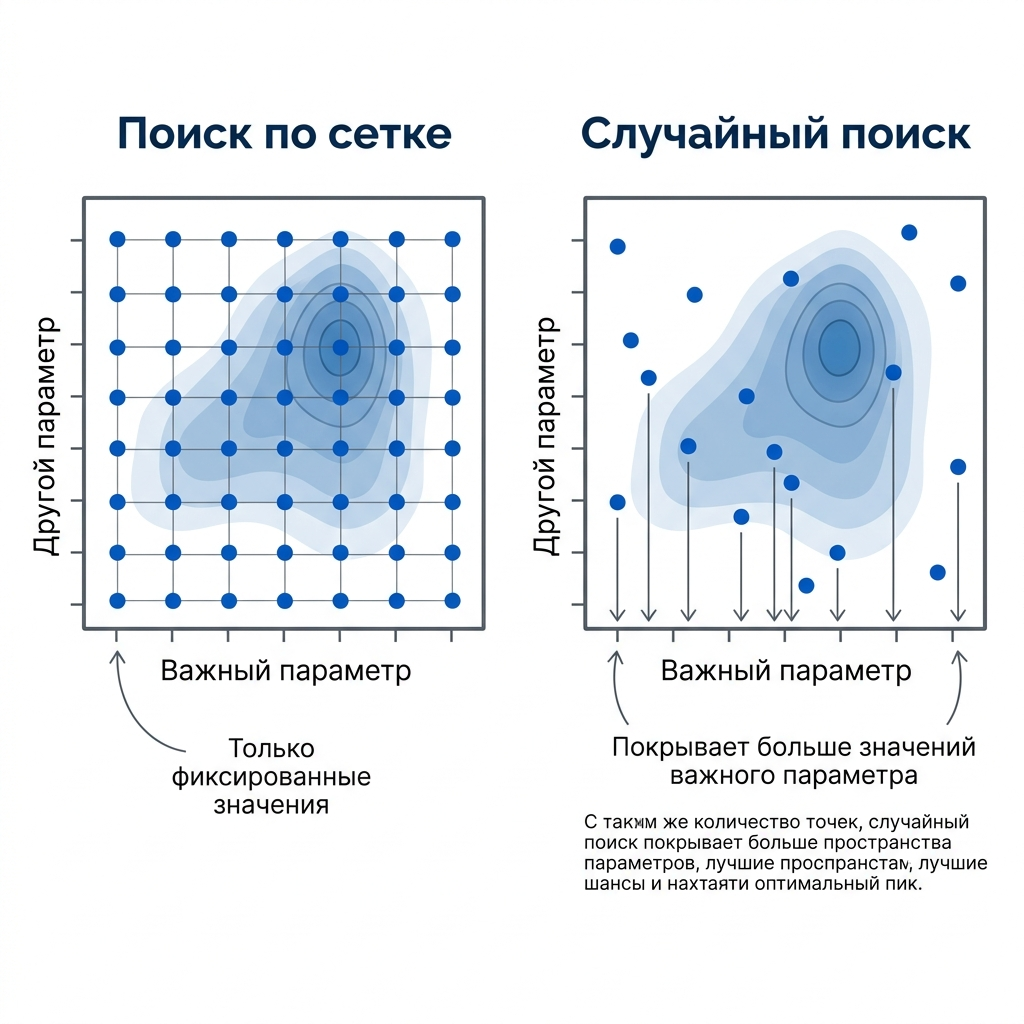
\includegraphics[width=0.8\textwidth]{grid_vs_random.png}
    \caption{Сравнение Grid Search и Random Search.}
\end{figure}

\subsection{Продвинутые методы}
\begin{itemize}
    \item \textbf{Байесовская оптимизация}: Строит вероятностную (суррогатную) модель функции потерь. Для выбора следующей точки используется \textbf{acquisition function} (функция полезности), которая балансирует между \textit{exploration} (исследование точек с большой дисперсией модели) и \textit{exploitation} (исследование точек с высоким ожидаемым качеством). Пример: $\alpha(x) = \mu(x) + \beta\sigma(x)$.
    \item \textbf{Population Based Training (PBT)}: Метод, объединяющий эволюционные алгоритмы и параллельное обучение. Процедура \texttt{exploit()}: если у модели низкое качество, её веса заменяются весами лучшей модели популяции. Процедура \texttt{explore()}: добавление случайного шума в гиперпараметры после перезаписи весов.
    \item \textbf{Алгоритм TPE (Tree-structured Parzen Estimator)}: Продвинутый вариант байесовской оптимизации, используемый в Hyperopt и Optuna.
\end{itemize}

\begin{figure}[h]
    \centering
    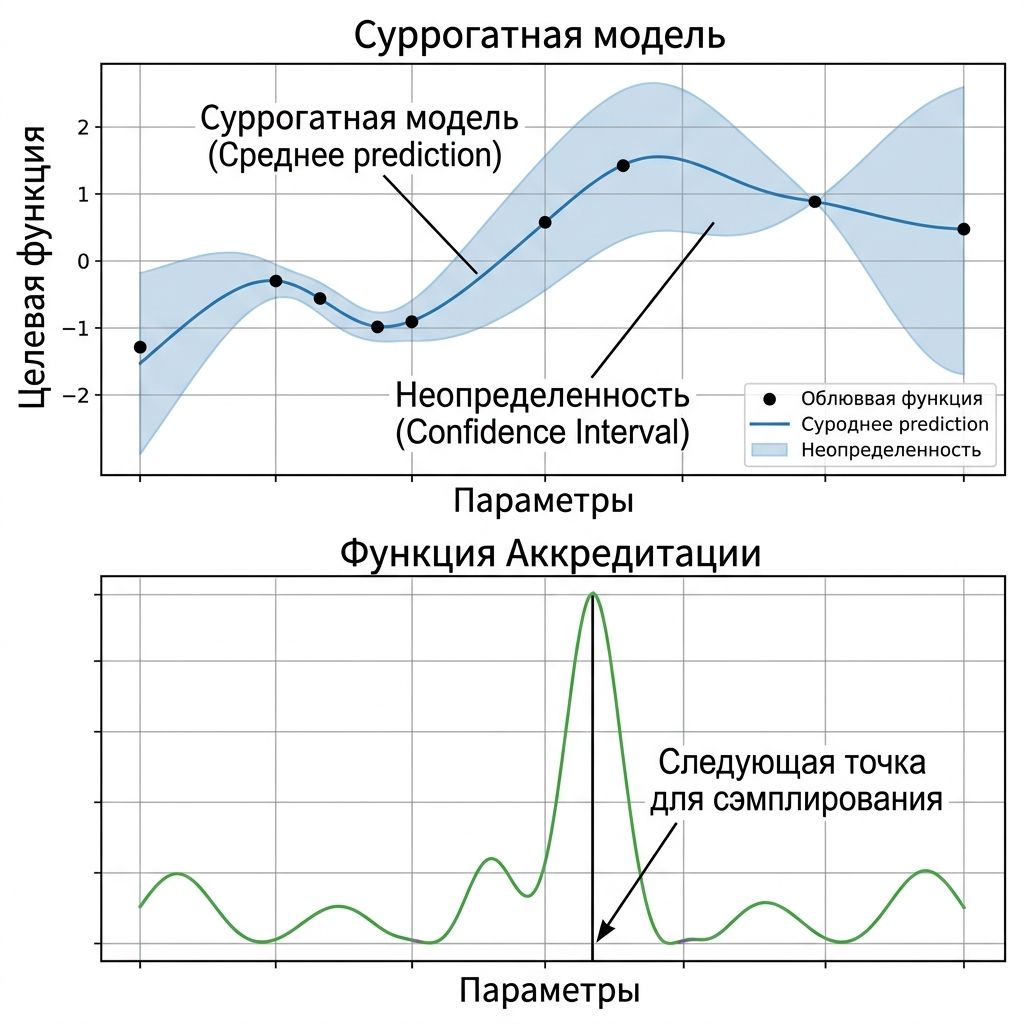
\includegraphics[width=0.7\textwidth]{bayesian_opt.png}
    \caption{Интуиция байесовской оптимизации.}
\end{figure}

\subsection{Опенсорс-библиотеки}
\begin{longtable}{lp{0.7\textwidth}}
\toprule
\textbf{Библиотека} & \textbf{Особенности} \\
\midrule
Scikit-learn & Базовые GridSearchCV и RandomizedSearchCV. \\
Hyperopt & Классика для метода TPE. \\
Optuna & Самая современная: define-by-run, быстрая, отличная визуализация. \\
skopt & Байесовская оптимизация с интерфейсом sklearn. \\
Keras Tuner & Инструмент для подбора архитектур нейросетей. \\
\bottomrule
\end{longtable}

\antigravity{Начинай всегда с Random Search, чтобы быстро прощупать почву. Если задача критически важна — переходи на Optuna.}

\end{document}
